%% Source Template:
%% Copyright (C) 2014 by Pascal Richter, Elena Botoeva, Richard Barnard, and Dirk Surmann
%% 
%% This file may be distributed and/or modified under the
%% conditions of the LaTeX Project Public License, either
%% version 2.0 of this license or (at your option) any later
%% version. The latest version of this license is in:
%% 
%% http://www.latex-project.org/lppl.txt
%% 
%% and version 2.0 or later is part of all distributions of
%% LaTeX version 2013/12/01 or later.
%% 

\documentclass[20pt, a1paper, portrait, margin=0mm, innermargin=8mm,
               blockverticalspace=8mm,colspace=5mm, subcolspace=0mm]
               {tikzposter}

% Choose Layout
\usetheme{Autumn}

% Additonal packages
\usepackage{wrapfig}
\usepackage{floatflt}
\usepackage{multicol}
\usepackage{placeins}
\usepackage[T1]{fontenc}
\usepackage{natbib}

% Set block style
\useblockstyle[titlewidthscale=1, bodywidthscale=1, titlecenter,
    titleoffsetx=0pt, titleoffsety=1pt, bodyoffsetx=0pt, bodyoffsety=25pt,
    bodyverticalshift=0pt, roundedcorners=5, linewidth=0.4cm,
    titleinnersep=8mm, bodyinnersep=8mm]{Default}

\usetitlestyle[titletoblockverticalspace=8mm]{Filled}

\tikzposterlatexaffectionproofoff


% Header
\title{\textcolor{colorThree}{\fontsize{2.3cm}{1em}\selectfont 
       Searching for signals in noise}}

\author{Gregory Ashton, supervised by D.I. Jones \& R. Prix \\
    {\Large G.Ashton@soton.ac.uk}}

\institute{University of Southampton }

\begin{document}

 % Title block with title, author, logo, etc.
\maketitle

\newcommand{\model}{\mathrm{model}}
\newcommand{\data}{\mathrm{data}}



 %\block{Introduction}{
%}
\begin{columns}
 % FIRST column
\newcommand{\mycolwidth}{0.5}
\column{\mycolwidth}
\block[]{I: Motivations}{
Astrophysics contains a huge number of interesting observed phenomena, let alone
those that we have yet to see. The problem we often have is that 
that our observations are in a low signal to noise regime; this can mean
several models can explain the observed data. 

In this poster we discuss a method for quantitatively assessing how well several
models fit some data. The aim being to decide, eventually, given the observed 
data which astrophysical model do we think is most likely.

}



 % SECOND column
\column{\mycolwidth}

\block{II: Bayesian Data Analysis}{
While many methods exist for comparing some models, an intuitive approach can
be found by using Bayes rule
\begin{equation}
    p(\model|\data) = p(\data|\model) \frac{p(\model)}{p(\data)}
    \label{eqn: bayes}
\end{equation}
where by $P(\model|\data)$ we mean "The probability of $\model$, given that 
we have observed some $\data$.

}

\end{columns}

\block{III: Model comparison}{
The issue with Bayes rule as written in eqn.(\ref{eqn: bayes}) is that 
$p(\data)$ is often difficult, or even impossible to define. Instead, we can
compare two models, say $M_{A}$ and $M_{B}$ by looking at the ratio
\begin{equation}
    \frac{p(M_{A}|\data)}{p(M_{B}|\data)} = 
    \frac{p(\data| M_{B})}{p(\data|M_{A})}
    \frac{p(M_{A})}{p(M_{B})}
\end{equation}
This ratio can directly be interpreted as the 'odds ratio', or how much more
we should believe model $A$ of $B$ given the data. The last fraction reflects
our prior knowledge about the two models. Unless we have a strong reason to
believe otherwise this is generally set to unity: $p(M_{A}) = p(M_{B})$.
}

\begin{columns}
\newcommand{\mycolwidth}{0.5}
\column{\mycolwidth}

\block{IV: Signals in noise}{
The key to data analysis is to define our 'likelihood' function: the
probability of the data given the model $p(\mathrm{data}|\mathrm{model})$. To 
calculate this we must first assume that the observed data is the sum of a
a deterministic signal and a central Gaussian noise process. That is we can
write the observed data as
\begin{equation}
    W(t) = f(t; \vec{\theta}) + n(t; \sigma).
\end{equation}
Here $f(t; \vec{\theta})$ is the signal model with parameters $\vec{\theta}$,
while $n(t; \sigma)$ is the noise process with strength $\sigma$. 
If we subtract the signal model (with the correct parameters) from the observed
data we should be left with Gaussian noise:
$W(t) - f(t; \vec{\theta}) = n(t; \sigma)$.
Then the probability of a single observed data point at $t_{i}$
\begin{equation}
    p(W(t_{i})|\mathrm{model}, \vec{\theta}, \sigma) = \frac{1}{\sqrt{2\pi\sigma}}e^{-\frac{(W(t_{i}) - f(t_{i})}{2\sigma^{2}}}
\end{equation}
Here the model, and hence the function $f(t)$, are yet to be determined. Given
a sequence of $N$ observations (e.g. some data) we can compute the likelihood
function as
\begin{equation}
    p(\mathrm{data}|\mathrm{model}, \vec{\theta}, \sigma) = \prod_{i=1}^{N}p(W(t_{i})|\mathrm{model}), \vec{\theta}, \sigma
    \label{eqn: likelihood}
\end{equation}
}

\column{\mycolwidth}
\block[]{V: Example}{

%\begin{wrapfigure}[8]{r}{0.8\linewidth}
%    \vspace{-10mm}
%\begin{tikzfigure}
%    \centering
%    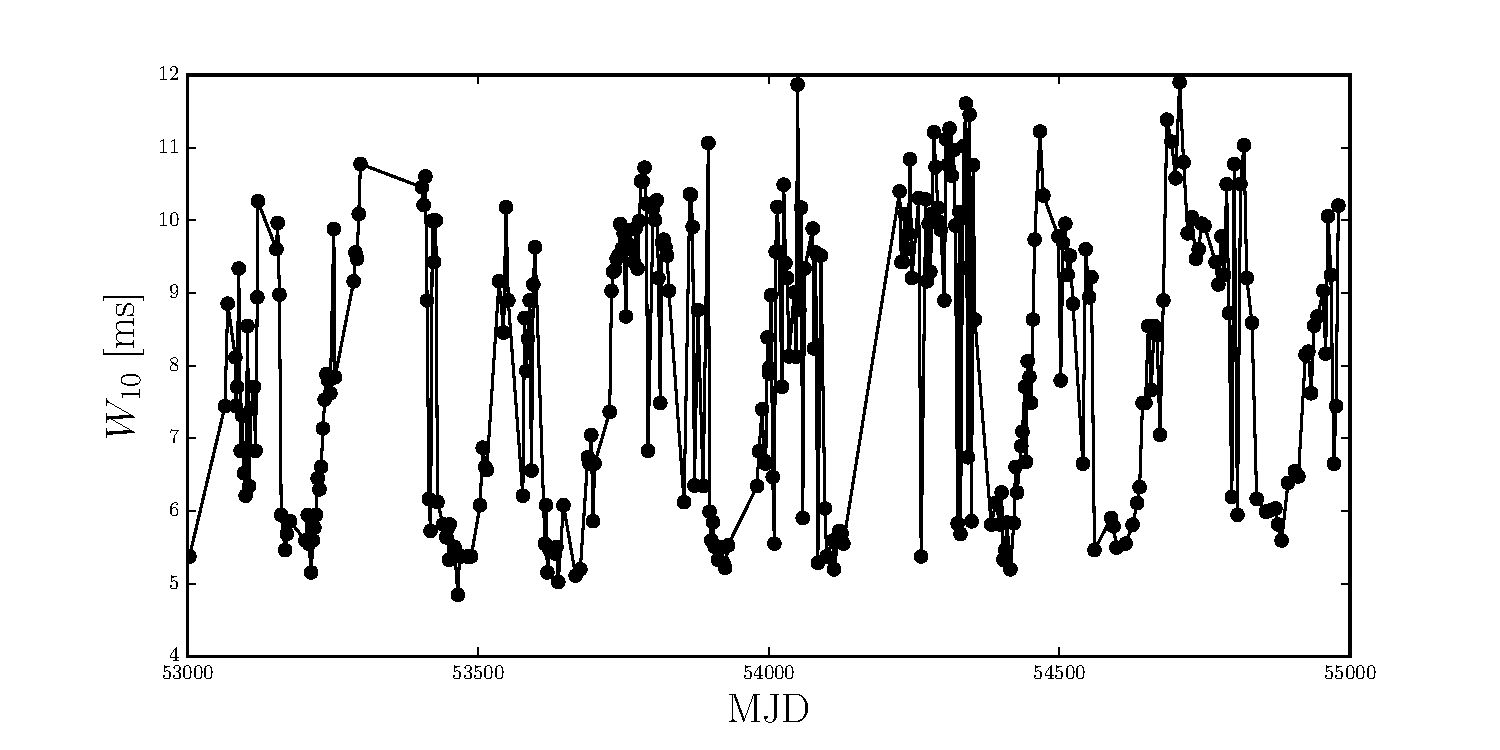
\includegraphics[width=0.33\textwidth]{img/raw_data}
%\end{tikzfigure}
%\end{wrapfigure}

To illustrate how we can apply Bayesian data analysis consider the data
shown in the figure below. This is a plot of the measured beam width
of pulsar B1828-11 showing a distinct periodic behaviour. This data was 
originally published in figure 5 of [1], we are thankful
to the original authors for allowing us access to this data.

\begin{tikzfigure}
    \centering
    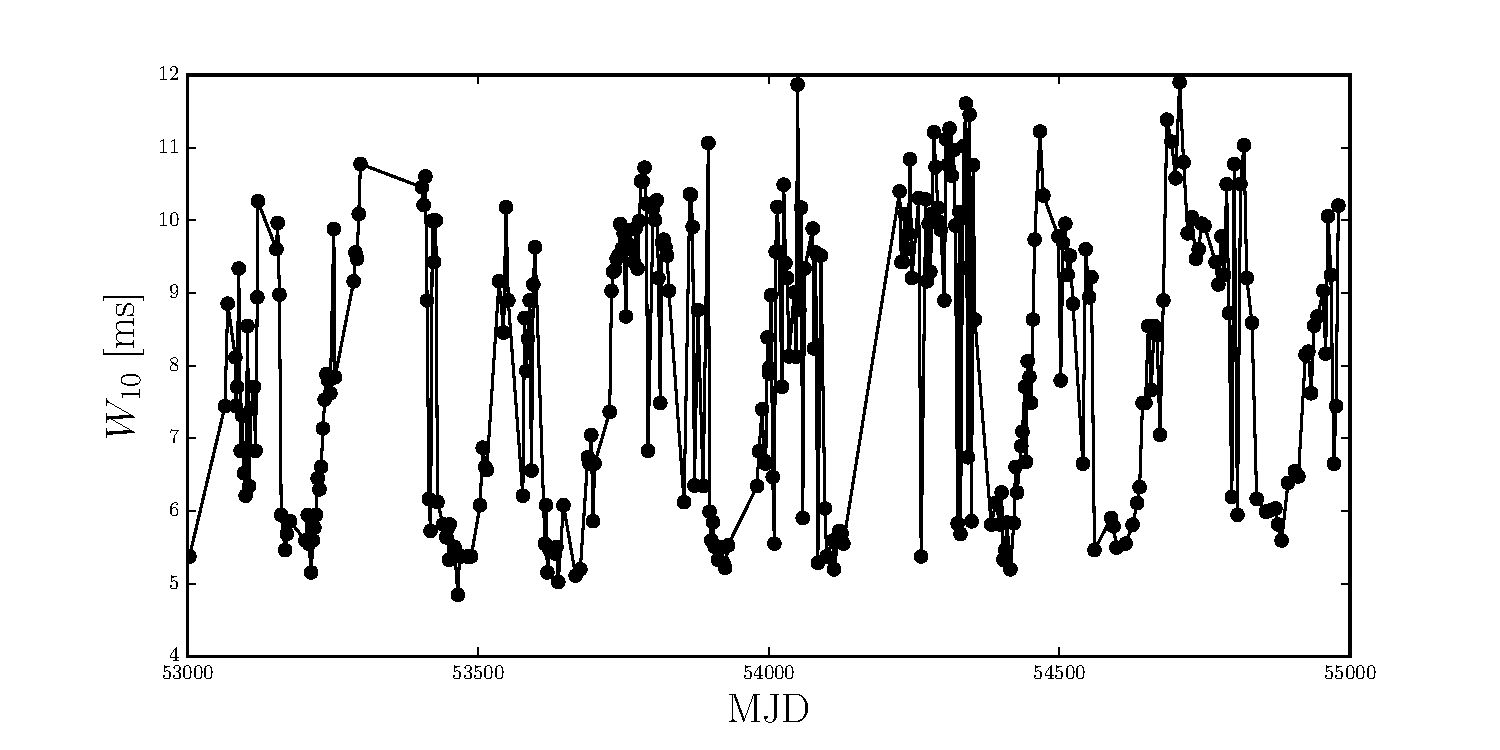
\includegraphics[width=0.33\textwidth]{img/raw_data}
\end{tikzfigure}

Prior to this paper, slow periodic modulation of the spin-down was cited as
evidence for precession in this pulsar. Clearly the beam width is also being 
modulated at this same time-scale. The authors argue that the beam width is
not smoothly varying between, but instead \emph{switching}. This has important
implications for neutron star physics.\\

\footnotesize
[1] Lyne, A., Hobbs, G., Kramer, M., Stairs, I., and Stappers, B. (2010). 
\emph{Switched Magnetospheric Regulation of Pulsar Spin-Down.} Science, 329:408–.
}

\end{columns}

\begin{columns}

\column{0.5}
\block[]{VI: Model A}{
The simplest model we can propose to explain the periodic features is a simple
trig. function. This does not capture all of the physics of alternative models,
but nevertheless will test the assumption that $W_{10}$ switches instantaneously
between two values. The signal function for this model is
\begin{equation}
    f(t; W_{0}, A, f, \phi_{0}) = W_{0} + A\sin(2\pi f t + \phi_{0}) 
    \label{eqn: A}
\end{equation}
}

\column{0.5}
\block[]{VII: Model B}{
The model proposed by the authors can be captured by a simple square wave. We
then make an assumption that the observed data is the sum of a square wave and
noise.
\begin{equation}
    g(t; W_{0}, A, f, \phi_{0}) = W_{0} + \mathrm{square}(t\; W_{0}, A, f, \phi_{0}) 
    \label{eqn: B}
\end{equation}
}
\end{columns}

\begin{columns}
\newcommand{\mycolwidth}{0.5}
\column{\mycolwidth}

\block{VIII: Marginalisation and odds ratio}{
Plugging the model functions \ref{eqn: A} and \ref{eqn: B} into the likelihood
\ref{eqn: likelihood} we have $P(\data| M_{i}, \vec{\theta}, \sigma)$. The next
step is to marginalise over all the model parameters:

\begin{equation}
    p(\data)| M_{i}) = \int \int p(\data | M_{i}, \vec{\theta}, \sigma) p(\vec{\theta}) p(\sigma) d\vec{\theta}d\sigma
\end{equation}

Often this integral will be unfeasible analytically, instead we can turn to 
numerical method such as MCMC and nested sampling.
}

\column{\mycolwidth}
\block{IX: Results}{
The observed beam width data was tested with both a sinusoidal model and a
square-wave model. We computed the marginal likelihoods using MCMC software
\emph{dan.iel.fm/emcee}. This resulted in an odds ratio:
\begin{equation}
    \log_{10}\left(\frac{p(M_{A}| \data)}{p(M_{B}| \data)}\right) = -6
\end{equation}
This establishes that the square wave model proposed by the authors significantly
out performs a sinusoidal model. We are currently in the process of exploring
more physical models to further probe the assumptions.

}


\end{columns}

\end{document}



\endinput
%%
